\documentclass{revtex4}

\usepackage{amsmath}
\usepackage{amsbsy}
\usepackage{amssymb}
\usepackage{graphicx}
\usepackage{bm,ulem,color}
\usepackage{natbib}


\providecommand{\dv}{\bm{\nabla}\cdot}
\providecommand{\curl}{\bm{\nabla}\times}

\providecommand{\tensor}[1]{ \underline{\bm{\mathsf{#1}}}}

\providecommand{\grad}{\bm{\nabla}}

\newcommand{\dg}{\cdot\grad}\newcommand{\collop}[1][f_s]{\ensuremath{{C}\hspace{-0.5mm}\left[#1\right]}}

\newcommand{\vth}[1][s]{\ensuremath{v_{\mathrm{th}_#1}}}
\newcommand{\vt}{\ensuremath{v_{\mathrm{th}}}}
\newcommand{\pd}[2]{\ensuremath{ \frac{\partial #1} {\partial #2} } }
\newcommand{\inpd}[2]{\ensuremath{ \infrac{\partial #1} {\partial #2} } }
\newcommand{\gyror}[1]{\ensuremath{ {\left< #1 \right>}_{\bm{r}}}}
\newcommand{\ensav}[1]{\ensuremath{ {\left< #1 \right>}_{\mathrm{turb}}}}  % Ensemble averaging
\newcommand{\fav}[1]{\ensuremath{\left< #1 \right>_{\psi}}} % Flux surface averaging
\newcommand{\gyroR}[1]{\ensuremath{{\left< #1 \right>}_{\bm{R}}}}

\providecommand{\eqref}[1]{Eq.\ (\ref{#1})}
\newcommand{\eqsref}[2]{Eqs.\ (\ref{#1}) and (\ref{#2})}
\newcommand{\eqsdash}[2]{Eqs.\ (\ref{#1})--(\ref{#2})}
\newcommand{\Secref}[1]{Section\ \ref{#1}}
\newcommand{\secref}[1]{Sec.\ \ref{#1}}
\newcommand{\apref}[1]{Appendix\ \ref{#1}}
\providecommand{\Apref}[1]{Appendix\ \ref{#1}}
\newcommand{\Figref}[1]{Fig.\ \ref{#1}}
\providecommand{\Tref}[1]{Table.\ \ref{#1}}

\providecommand{\Or}[1]{\mathcal{O}#1}
\providecommand{\Eref}[1]{Equation\ (\ref{#1})}
\providecommand{\eref}[1]{(\ref{#1})}


\newcommand{\uv}[1]{\bm{\hat{#1}}} % uv = unit vector
\newcommand{\pb}[2]{\left\{ {#1} \middle., {#2} \right\}} % pb = poisson bracket

% Change the following commands to alter the notation of the document.

\newcommand{\tor}{\phi} % toroidal angle
\newcommand{\gyr}{\vartheta} % gyroangle
\newcommand{\pot}{\varphi} % electrostatic potential
\newcommand{\fpot}{\Phi} % Flow potential
\newcommand{\pol}{\theta} % Poloidal angle (straight field)
\newcommand{\gkeps}{\epsilon} % Rho over L, gyrokinetic epsilon
\newcommand{\aspect}{\epsilon} % Inverse aspect ratio
\newcommand{\energy}[1][s]{{{\varepsilon}_#1}} % Energy Variable
\newcommand{\denergy}[1][s]{{\dot{\varepsilon}}_{#1}}
\newcommand{\torflux}{\Psi} % Toroidal flux
\newcommand{\source}[1][s]{\ensuremath{{{{S}}_{#1}}}} % General Source
\newcommand{\gkupot}{\delta \pot'}
\newcommand{\gkpot}{\chi}
\newcommand{\psistar}[1][s]{{\psi^*_#1}}
\newcommand{\psistardot}[1][s]{{\dot{\psi}^*_#1}}
\newcommand{\magmom}[1][s]{\mu_#1}
\newcommand{\dmu}[1][s]{\dot{\mu}_#1}
\newcommand{\jacob}{\mathcal{J}}
%\newcommand{\idmat}{\bm{\underline{\mathbb{I}}}} % Identity Matrix
\newcommand{\tu}{\hat{u}_{\parallel s}}

\newcommand{\ddR}[2][s]{\pd{#2}{\bm{R}_{#1}}}
\newcommand{\dgR}[2][s]{\cdot\ddR[#1]{#2}}

\newcommand{\tcite}[1]{Ref.\ \onlinecite{#1}}
\providecommand{\tensor}[1]{ {\bm{\mathsf{#1}}}}
\newcommand{\viscosity}[1][s]{\tensor{\Pi}_#1}
\newcommand{\idmat}{\tensor{I}}
\newcommand{\ParticleFlux}[1][s]{\Gamma_{#1}}
\newcommand{\HeatFlux}[1][s]{q_{#1}}
\newcommand{\MomentumFlux}[1][s]{\pi^{(\psi\tor)}_{#1}}
\newcommand{\TotMomFlux}{{\pi}^{(\psi\tor)}_{\mathrm{tot}}}
\newcommand{\inertia}{J}
\newcommand{\accel}[1][s]{\bm{a}_{#1}}
\newcommand{\daccel}[1][s]{\delta \bm{a}_{#1}}
% partial with respect to time at constant psi
\newcommand{\ddtpsi}{\left.\pd{}{t}\right|_{\psi}}
% IOP 
\newcommand{\oxford}{
Rudolf Peierls Centre for Theoretical Physics, University of Oxford, Oxford OX1 3PU, UK
}

\newcommand{\culham}{
EURATOM/CCFE Fusion Association, Culham Science Centre, Abingdon OX14 3DB, UK
}

\newcommand{\imperial}{
Blackett Laboratory, Imperial College, London SW7 2AZ, UK
}

\newcommand{\maryland}{
Department of Physics, University of Maryland, College Park, MD 20742-4111, USA
}

\newcommand{\ireap}{
Institute of Research in Electronics and Applied Physics, University of Maryland, College Park, MD 20742, USA
}

\newcommand{\llnl}{
Lawrence Livermore National Laboratory, Livermore, CA 94550, USA
}

\newcommand{\merton}{
Merton College, Oxford, OX1 4JD, UK
}

\newcommand{\mitpsfc}{
Plasma Science and Fusion Center, Massachusetts Institute of Technology, Cambridge, MA 02139, USA
}

\newcommand{\princeton}{
Princeton Plasma Physics Laboratory, Princeton, NJ 08543, USA
}

\newcommand{\pcts}{
Princeton Center for Theoretical Science, Princeton University, Princeton, NJ 08544, USA
}

\newcommand{\chalmers}{
Department of Physics, Chalmers University of Technology, G\"oteborg, SE-41296, Sweden
}

\newcommand{\ippgreifs}{
Max-Planck-Institut f\"ur Plasmaphysik, 17491 Greifswald, Germany
}

\newcommand{\neilsbohr}{
Neils Bohr International Academy, University of Copenhagen, Copenhagen, Denmark
}

\newcommand{\wint}{\int\hspace{-1.25mm} d^3 \bm{w}}
\newcommand{\Fneo}[1][s]{F^{\mathrm{(nc)}}_{#1}}
\newcommand{\FE}{F^{\mathrm{(E)}}_{s}}
\newcommand{\Fnct}{\tilde{F}^{\mathrm{(nc)}}_{s}}
\newcommand{\Fstar}[1][s]{F^{*}_{1#1}}
\newcommand{\Esource}[1][s]{S^{({E})}_{#1}}
\newcommand{\Psource}[1][s]{S^{({n})}_{#1}}
\newcommand{\Msource}{S^{({\omega})}}
\newcommand{\FreeEnergy}{W}
\newcommand{\perpav}[1]{\left<#1\right>_\perp}
\newcommand{\timeav}[1]{\left<#1\right>_T}
\newcommand{\injpow}{P_{\mathrm{inj}}}
\newcommand{\entropy}[1][]{\widetilde{H}_{#1}}
\newcommand{\MeanEntropy}[1][]{H_{#1}}
\newcommand{\deltaEntropy}[1][]{\delta H_{#1}}
\newcommand{\entropyflux}{\bm{\Gamma}^{({H})}}
\newcommand{\infrac}[2]{ \left.{#1}\middle/{#2}\right. }
\newcommand{\binfrac}[2]{\left(\infrac{#1}{#2}\right)}
\newcommand{\CollEnergy}[1][s]{C^{{(E)}}_#1}
\newcommand{\ViscousHeat}[1][s]{P^{\mathrm{visc}}_#1}
\newcommand{\JouleHeat}[1][s]{P^{\mathrm{Ohm}}_#1}
\newcommand{\PotEng}[1][s]{P^{\mathrm{pot}}_#1}
\newcommand{\CompHeat}[1][s]{P^{\mathrm{comp}}_#1}
\newcommand{\TurbInj}[1][s]{P^{\mathrm{drive}}_#1}
\newcommand{\TurbColl}[1][s]{P^{\mathrm{diss}}_#1}
\newcommand{\TurbPow}[1][s]{P^{\mathrm{turb}}_#1}
\newcommand{\EMViscosity}{\pi_{\mathrm{EM}}^{(\psi\tor)}}
\newcommand{\NeoMomFlux}[1][s]{\pi^{\mathrm{(nc)}}_{#1}}
\newcommand{\ClassMomFlux}[1][s]{\pi^{\mathrm{(cl)}}_{#1}}
\newcommand{\vchi}{\bm{V}_\chi}
\newcommand{\vchiR}{\gyroR{\vchi}}
\newcommand{\vdrift}[1][s]{\bm{V}_{\mathrm{D}#1}}
\newcommand{\GammaTurb}{\Gamma_{s}^{\mathrm{turb}}}
\newcommand{\QTurb}{q_{s}^{\mathrm{turb}}}
\newcommand{\PiTurb}{\pi_{s}^{\mathrm{turb}}}
\newcommand{\EProd}{C^{\mathrm{(H)}}}
\newcommand{\Rentropyflux}{\Gamma^{({H})}}
\newcommand{\JUflux}{\Gamma^{{(U)}}}
\newcommand{\CollEntropy}{C^{{(H)}}}
\newcommand{\EntropySource}{S^{{(H)}}}
\newcommand{\DebyeLength}{\lambda_{\mathrm{De}}}
\newcommand{\NotN}[1][s]{N_{#1}}
\newcommand{\massratio}{\delta}

\newcommand{\delB}{{\ensuremath{\delta\bm{B}}}}
\newcommand{\delBp}{{\ensuremath{\delta B_\parallel}}}
\newcommand{\delBpN}[1]{{\ensuremath{\delta B_\parallel^{(#1)}}}}
\newcommand{\delAp}{{\ensuremath{\delta A_\parallel}}}
\newcommand{\delApN}[1]{{\ensuremath{\delta A_\parallel^{(#1)}}}}
\newcommand{\delE}{{\ensuremath{\delta\bm{E}}}}
\newcommand{\delA}{{\ensuremath{\delta\bm{A}}}}
\newcommand{\delj}{{\ensuremath{\delta\bm{j}}}}
\newcommand{\delpot}{{\delta\pot}}
\newcommand{\MagDelB}{{\delta B}} \newcommand{\bhat}{{\widetilde{\bm{b}}}}

\newcommand{\MeanB}{{\bm{B}}}
\newcommand{\MeanE}{{\bm{E}}}
\newcommand{\MeanMagB}{{B}}
\newcommand{\Meanb}{{\bm{b}}}
\newcommand{\Meanj}{{\bm{j}}}

\newcommand{\Efield}{{\widetilde{\bm{E}}}}
\newcommand{\Bfield}{{\widetilde{\bm{B}}}}
\newcommand{\MagBfield}{{\widetilde{B}}}

\newcommand{\current}{{\widetilde{\bm{j}}}}
\newcommand{\chargedens}{{\widetilde{\varrho}}}
\newcommand{\Apot}{{\widetilde{\bm{A}}}}
\newcommand{\Epot}{{\widetilde{\pot}}}
\newcommand{\MeanA}{{\bm{A}}}
\newcommand{\MeanPot}{{\pot}}

% Averages and abbreviations for paper 2
\newcommand{\bav}[1]{\left<#1\right>_{\parallel}}
\newcommand{\veff}{\bm{u}_{\mathrm{eff}}}
\newcommand{\fluctfav}[1]{\left<#1\right>_{\tilde\psi}}

\newcommand{\upar}[1][e]{\delta u_{\parallel #1}}
\newcommand{\tpsi}{\tilde{\psi}}
\newcommand{\talpha}{\tilde{\alpha}}
\newcommand{\tl}{\tilde{l}}
\newcommand{\ddttwiddles}[1][]{\left.\pd{#1}{t}\right|_{\tilde{\psi},\tilde{\alpha},\tilde{l}}}
\newcommand{\qpar}{\delta q_{\parallel e}}

\newcommand{\FHat}[1][s]{\widehat{F}_{1#1}}
\newcommand{\angvel}{\omega}
\newcommand{\cycfreq}[1][s]{\Omega_{#1}}

\newcommand{\ExEnergy}[1][s]{\widetilde{\varepsilon}_{#1}}
\newcommand{\ExMagmom}[1][s]{\widetilde{\mu}_{#1}}
\newcommand{\ExGyr}{\widetilde{\gyr}}
\newcommand{\dExGyr}{\dot{\widetilde{\gyr}}}
\newcommand{\dExenergy}[1][s]{{\dot{\widetilde{\varepsilon}}}_{#1}}
\newcommand{\magmomN}[2][s]{{\mu}_{#2#1}}
\newcommand{\mmbar}[2][s]{\overbar{\magmomN[#1]{#2}}}
\newcommand{\dmmbar}[2][s]{\overbar{\delta\magmomN[#1]{#2}}}
\newcommand{\vA}{v_{\mathrm{A}}} % Alfvèn velocity
\newcommand{\cS}{c_{\mathrm{s}}} % Alfvèn velocity
\newcommand{\bpol}{\beta_{\mathrm{pol}}}
\providecommand{\omstar}[1][]{\ensuremath{\omega_{*#1}}}
%\newcommand{\Tref}[1]{Table~\ref{#1}}
%\newcommand{\tref}[1]{table~\ref{#1}}

\newcommand{\chempot}[1][s]{\Upsilon_{#1}}
\newcommand{\quantconc}[1][s]{n_{\mathrm{Q}#1}}

\newcommand{\vpsi}{\bm{V}_\psi}

\newcommand{\tw}{\widetilde{\bm{w}}}
\newcommand{\twint}{\int d^{3}\widetilde{\bm{w}}}
\newcommand{\Magtw}{\widetilde{{w}}}

\newcommand{\dgt}{\cdot\widetilde{\nabla}_\perp}

\newcommand{\MaxVDrift}{\widehat{\bm{V}}_D}
\newcommand{\ddtpsitwiddles}{\left.\pd{ }{t}\right|_{\tpsi}}
\newcommand{\Pturb}{P^{\mathrm{turb}}_e}
\newcommand{\Pmean}{P^{\mathrm{mean}}_e}
\newcommand{\tvp}{\tilde{V}'}
\newcommand{\tee}{\tilde{\varepsilon}_e}
\newcommand{\delNe}{\overbar{\delta n}_e}
\newcommand{\delTe}{\overbar{\delta T}_e}

\newcommand{\delEnt}[1][s]{{\Delta S_{#1}}}

\newcommand{\overbar}[1]{\mkern 1.5mu\overline{\mkern-1.5mu#1\mkern-1.5mu}\mkern 1.5mu}
\newcommand{\nustar}[1][e]{\nu^{*}_{#1}}
\newcommand{\shat}{\hat{s}}

\newcommand{\lincol}[1][\cdot]{\ensuremath{{C}_{L}\hspace{-0.5mm}\left[#1\right]}}
\newcommand{\npol}{\ensuremath{n^{\mathrm{pol}}_s}}
\newcommand{\poldrift}{\ensuremath{\bm{V}^{\mathrm{pol}}_s}}

\newcommand{\ash}{\ensuremath{\mathrm{ash}}}

\newcommand{\rhos}{\ensuremath{\rho_{\mathrm{s}}}} % Sound radius
\newcommand{\cs}{\ensuremath{c_{\mathrm{s}}}} % Sound speed

\newcommand{\gstwo}{{\ttfamily GS2}}
\newcommand{\trinity}{{\ttfamily TRINITY}}

\RequirePackage{amsmath}
\makeatletter
\newcommand*\rel@kern[1]{\kern#1\dimexpr\macc@kerna}
\newcommand*\widebar[1]{%
  \begingroup
  \def\mathaccent##1##2{%
    \rel@kern{0.8}%
    \overline{\rel@kern{-0.8}\macc@nucleus\rel@kern{0.2}}%
    \rel@kern{-0.2}%
  }%
  \macc@depth\@ne
  \let\math@bgroup\@empty \let\math@egroup\macc@set@skewchar
  \mathsurround\z@ \frozen@everymath{\mathgroup\macc@group\relax}%
  \macc@set@skewchar\relax
  \let\mathaccentV\macc@nested@a
  \macc@nested@a\relax111{#1}%
  \endgroup
}
\makeatother


\newcommand{\collop}[1][f_s]{\ensuremath{{C}\hspace{-0.5mm}\left[#1\right]}}
\newcommand{\vth}[1][s]{\ensuremath{v_{\mathrm{th}_#1}}}
\newcommand{\vt}{\ensuremath{v_{\mathrm{th}}}}
\newcommand{\pd}[2]{\ensuremath{ \frac{\partial #1} {\partial #2} } }
\newcommand{\inpd}[2]{\ensuremath{ \infrac{\partial #1} {\partial #2} } }
\newcommand{\gyror}[1]{\ensuremath{ {\left< #1 \right>}_{\bm{r}}}}
\newcommand{\ensav}[1]{\ensuremath{ {\left< #1 \right>}_{\mathrm{turb}}}}  % Ensemble averaging
\newcommand{\fav}[1]{\ensuremath{\left< #1 \right>_{\psi}}} % Flux surface averaging
\newcommand{\gyroR}[1]{\ensuremath{{\left< #1 \right>}_{\bm{R}}}}

\providecommand{\eqref}[1]{Eq.\ (\ref{#1})}
\newcommand{\eqsref}[2]{Eqs.\ (\ref{#1}) and (\ref{#2})}
\newcommand{\eqsdash}[2]{Eqs.\ (\ref{#1})--(\ref{#2})}
\newcommand{\Secref}[1]{Section\ \ref{#1}}
\newcommand{\secref}[1]{Sec.\ \ref{#1}}
\newcommand{\apref}[1]{Appendix\ \ref{#1}}
\providecommand{\Apref}[1]{Appendix\ \ref{#1}}
\newcommand{\Figref}[1]{Fig.\ \ref{#1}}
\providecommand{\Tref}[1]{Table.\ \ref{#1}}

\providecommand{\Or}[1]{\mathcal{O}#1}
\providecommand{\Eref}[1]{Equation\ (\ref{#1})}
\providecommand{\eref}[1]{(\ref{#1})}


\newcommand{\uv}[1]{\bm{\hat{#1}}} % uv = unit vector
\newcommand{\dg}{\cdot\nabla}      % dg = dot grad
\providecommand{\dv}{\nabla\cdot}
\providecommand{\curl}{\nabla\times}
\newcommand{\pb}[2]{\left\{ {#1} \middle., {#2} \right\}} % pb = poisson bracket

% Change the following commands to alter the notation of the document.

\newcommand{\tor}{\phi} % toroidal angle
\newcommand{\gyr}{\vartheta} % gyroangle
\newcommand{\pot}{\varphi} % electrostatic potential
\newcommand{\fpot}{\Phi} % Flow potential
\newcommand{\pol}{\theta} % Poloidal angle (straight field)
\newcommand{\gkeps}{\epsilon} % Rho over L, gyrokinetic epsilon
\newcommand{\aspect}{\epsilon} % Inverse aspect ratio
\newcommand{\energy}[1][s]{{{\varepsilon}_#1}} % Energy Variable
\newcommand{\denergy}[1][s]{{\dot{\varepsilon}}_{#1}}
\newcommand{\torflux}{\Psi} % Toroidal flux
\newcommand{\source}[1][s]{\ensuremath{{{{S}}_{#1}}}} % General Source
\newcommand{\gkupot}{\delta \pot'}
\newcommand{\gkpot}{\chi}
\newcommand{\psistar}[1][s]{{\psi^*_#1}}
\newcommand{\psistardot}[1][s]{{\dot{\psi}^*_#1}}
\newcommand{\magmom}[1][s]{\mu_#1}
\newcommand{\dmu}[1][s]{\dot{\mu}_#1}
\newcommand{\jacob}{\mathcal{J}}
%\newcommand{\idmat}{\bm{\underline{\mathbb{I}}}} % Identity Matrix
\newcommand{\tu}{\hat{u}_{\parallel s}}

\newcommand{\ddR}[2][s]{\pd{#2}{\bm{R}_{#1}}}
\newcommand{\dgR}[2][s]{\cdot\ddR[#1]{#2}}

\newcommand{\tcite}[1]{Ref.\ \onlinecite{#1}}
\providecommand{\tensor}[1]{ {\bm{\mathsf{#1}}}}
\newcommand{\viscosity}[1][s]{\tensor{\Pi}_#1}
\newcommand{\idmat}{\tensor{I}}
\newcommand{\ParticleFlux}[1][s]{\Gamma_{#1}}
\newcommand{\HeatFlux}[1][s]{q_{#1}}
\newcommand{\MomentumFlux}[1][s]{\pi^{(\psi\tor)}_{#1}}
\newcommand{\TotMomFlux}{{\pi}^{(\psi\tor)}_{\mathrm{tot}}}
\newcommand{\inertia}{J}
\newcommand{\accel}[1][s]{\bm{a}_{#1}}
\newcommand{\daccel}[1][s]{\delta \bm{a}_{#1}}
% partial with respect to time at constant psi
\newcommand{\ddtpsi}{\left.\pd{}{t}\right|_{\psi}}
% IOP 
\newcommand{\oxford}{
Rudolf Peierls Centre for Theoretical Physics, University of Oxford, Oxford OX1 3PU, UK
}

\newcommand{\culham}{
EURATOM/CCFE Fusion Association, Culham Science Centre, Abingdon OX14 3DB, UK
}

\newcommand{\imperial}{
Blackett Laboratory, Imperial College, London SW7 2AZ, UK
}

\newcommand{\maryland}{
Department of Physics, University of Maryland, College Park, MD 20742-4111, USA
}

\newcommand{\ireap}{
Institute of Research in Electronics and Applied Physics, University of Maryland, College Park, MD 20742, USA
}

\newcommand{\llnl}{
Lawrence Livermore National Laboratory, Livermore, CA 94550, USA
}

\newcommand{\merton}{
Merton College, Oxford, OX1 4JD, UK
}

\newcommand{\mitpsfc}{
Plasma Science and Fusion Center, Massachusetts Institute of Technology, Cambridge, MA 02139, USA
}

\newcommand{\princeton}{
Princeton Plasma Physics Laboratory, Princeton, NJ 08543, USA
}

\newcommand{\pcts}{
Princeton Center for Theoretical Science, Princeton University, Princeton, NJ 08544, USA
}

\newcommand{\chalmers}{
Department of Physics, Chalmers University of Technology, G\"oteborg, SE-41296, Sweden
}

\newcommand{\ippgreifs}{
Max-Planck-Institut f\"ur Plasmaphysik, 17491 Greifswald, Germany
}

\newcommand{\neilsbohr}{
Neils Bohr International Academy, University of Copenhagen, Copenhagen, Denmark
}

\newcommand{\wint}{\int\hspace{-1.25mm} d^3 \bm{w}}
\newcommand{\Fneo}[1][s]{F^{\mathrm{(nc)}}_{#1}}
\newcommand{\FE}{F^{\mathrm{(E)}}_{s}}
\newcommand{\Fnct}{\tilde{F}^{\mathrm{(nc)}}_{s}}
\newcommand{\Fstar}[1][s]{F^{*}_{1#1}}
\newcommand{\Esource}[1][s]{S^{({E})}_{#1}}
\newcommand{\Psource}[1][s]{S^{({n})}_{#1}}
\newcommand{\Msource}{S^{({\omega})}}
\newcommand{\FreeEnergy}{W}
\newcommand{\perpav}[1]{\left<#1\right>_\perp}
\newcommand{\timeav}[1]{\left<#1\right>_T}
\newcommand{\injpow}{P_{\mathrm{inj}}}
\newcommand{\entropy}[1][]{\widetilde{H}_{#1}}
\newcommand{\MeanEntropy}[1][]{H_{#1}}
\newcommand{\deltaEntropy}[1][]{\delta H_{#1}}
\newcommand{\entropyflux}{\bm{\Gamma}^{({H})}}
\newcommand{\infrac}[2]{ \left.{#1}\middle/{#2}\right. }
\newcommand{\binfrac}[2]{\left(\infrac{#1}{#2}\right)}
\newcommand{\CollEnergy}[1][s]{C^{{(E)}}_#1}
\newcommand{\ViscousHeat}[1][s]{P^{\mathrm{visc}}_#1}
\newcommand{\JouleHeat}[1][s]{P^{\mathrm{Ohm}}_#1}
\newcommand{\PotEng}[1][s]{P^{\mathrm{pot}}_#1}
\newcommand{\CompHeat}[1][s]{P^{\mathrm{comp}}_#1}
\newcommand{\TurbInj}[1][s]{P^{\mathrm{drive}}_#1}
\newcommand{\TurbColl}[1][s]{P^{\mathrm{diss}}_#1}
\newcommand{\TurbPow}[1][s]{P^{\mathrm{turb}}_#1}
\newcommand{\EMViscosity}{\pi_{\mathrm{EM}}^{(\psi\tor)}}
\newcommand{\NeoMomFlux}[1][s]{\pi^{\mathrm{(nc)}}_{#1}}
\newcommand{\ClassMomFlux}[1][s]{\pi^{\mathrm{(cl)}}_{#1}}
\newcommand{\vchi}{\bm{V}_\chi}
\newcommand{\vchiR}{\gyroR{\vchi}}
\newcommand{\vdrift}[1][s]{\bm{V}_{\mathrm{D}#1}}
\newcommand{\GammaTurb}{\Gamma_{s}^{\mathrm{turb}}}
\newcommand{\QTurb}{q_{s}^{\mathrm{turb}}}
\newcommand{\PiTurb}{\pi_{s}^{\mathrm{turb}}}
\newcommand{\EProd}{C^{\mathrm{(H)}}}
\newcommand{\Rentropyflux}{\Gamma^{({H})}}
\newcommand{\JUflux}{\Gamma^{{(U)}}}
\newcommand{\CollEntropy}{C^{{(H)}}}
\newcommand{\EntropySource}{S^{{(H)}}}
\newcommand{\DebyeLength}{\lambda_{\mathrm{De}}}
\newcommand{\NotN}[1][s]{N_{#1}}
\newcommand{\massratio}{\delta}

\newcommand{\delB}{{\ensuremath{\delta\bm{B}}}}
\newcommand{\delBp}{{\ensuremath{\delta B_\parallel}}}
\newcommand{\delBpN}[1]{{\ensuremath{\delta B_\parallel^{(#1)}}}}
\newcommand{\delAp}{{\ensuremath{\delta A_\parallel}}}
\newcommand{\delApN}[1]{{\ensuremath{\delta A_\parallel^{(#1)}}}}
\newcommand{\delE}{{\ensuremath{\delta\bm{E}}}}
\newcommand{\delA}{{\ensuremath{\delta\bm{A}}}}
\newcommand{\delj}{{\ensuremath{\delta\bm{j}}}}
\newcommand{\delpot}{{\delta\pot}}
\newcommand{\MagDelB}{{\delta B}} \newcommand{\bhat}{{\widetilde{\bm{b}}}}

\newcommand{\MeanB}{{\bm{B}}}
\newcommand{\MeanE}{{\bm{E}}}
\newcommand{\MeanMagB}{{B}}
\newcommand{\Meanb}{{\bm{b}}}
\newcommand{\Meanj}{{\bm{j}}}

\newcommand{\Efield}{{\widetilde{\bm{E}}}}
\newcommand{\Bfield}{{\widetilde{\bm{B}}}}
\newcommand{\MagBfield}{{\widetilde{B}}}

\newcommand{\current}{{\widetilde{\bm{j}}}}
\newcommand{\chargedens}{{\widetilde{\varrho}}}
\newcommand{\Apot}{{\widetilde{\bm{A}}}}
\newcommand{\Epot}{{\widetilde{\pot}}}
\newcommand{\MeanA}{{\bm{A}}}
\newcommand{\MeanPot}{{\pot}}

% Averages and abbreviations for paper 2
\newcommand{\bav}[1]{\left<#1\right>_{\parallel}}
\newcommand{\veff}{\bm{u}_{\mathrm{eff}}}
\newcommand{\fluctfav}[1]{\left<#1\right>_{\tilde\psi}}

\newcommand{\upar}[1][e]{\delta u_{\parallel #1}}
\newcommand{\tpsi}{\tilde{\psi}}
\newcommand{\talpha}{\tilde{\alpha}}
\newcommand{\tl}{\tilde{l}}
\newcommand{\ddttwiddles}[1][]{\left.\pd{#1}{t}\right|_{\tilde{\psi},\tilde{\alpha},\tilde{l}}}
\newcommand{\qpar}{\delta q_{\parallel e}}

\newcommand{\FHat}[1][s]{\widehat{F}_{1#1}}
\newcommand{\angvel}{\omega}
\newcommand{\cycfreq}[1][s]{\Omega_{#1}}

\newcommand{\ExEnergy}[1][s]{\widetilde{\varepsilon}_{#1}}
\newcommand{\ExMagmom}[1][s]{\widetilde{\mu}_{#1}}
\newcommand{\ExGyr}{\widetilde{\gyr}}
\newcommand{\dExGyr}{\dot{\widetilde{\gyr}}}
\newcommand{\dExenergy}[1][s]{{\dot{\widetilde{\varepsilon}}}_{#1}}
\newcommand{\magmomN}[2][s]{{\mu}_{#2#1}}
\newcommand{\mmbar}[2][s]{\overbar{\magmomN[#1]{#2}}}
\newcommand{\dmmbar}[2][s]{\overbar{\delta\magmomN[#1]{#2}}}
\newcommand{\vA}{v_{\mathrm{A}}} % Alfvèn velocity
\newcommand{\cS}{c_{\mathrm{s}}} % Alfvèn velocity
\newcommand{\bpol}{\beta_{\mathrm{pol}}}
\providecommand{\omstar}[1][]{\ensuremath{\omega_{*#1}}}
%\newcommand{\Tref}[1]{Table~\ref{#1}}
%\newcommand{\tref}[1]{table~\ref{#1}}

\newcommand{\chempot}[1][s]{\Upsilon_{#1}}
\newcommand{\quantconc}[1][s]{n_{\mathrm{Q}#1}}

\newcommand{\vpsi}{\bm{V}_\psi}

\newcommand{\tw}{\widetilde{\bm{w}}}
\newcommand{\twint}{\int d^{3}\widetilde{\bm{w}}}
\newcommand{\Magtw}{\widetilde{{w}}}

\newcommand{\dgt}{\cdot\widetilde{\nabla}_\perp}

\newcommand{\MaxVDrift}{\widehat{\bm{V}}_D}
\newcommand{\ddtpsitwiddles}{\left.\pd{ }{t}\right|_{\tpsi}}
\newcommand{\Pturb}{P^{\mathrm{turb}}_e}
\newcommand{\Pmean}{P^{\mathrm{mean}}_e}
\newcommand{\tvp}{\tilde{V}'}
\newcommand{\tee}{\tilde{\varepsilon}_e}
\newcommand{\delNe}{\overbar{\delta n}_e}
\newcommand{\delTe}{\overbar{\delta T}_e}

\newcommand{\delEnt}[1][s]{{\Delta S_{#1}}}

\newcommand{\overbar}[1]{\mkern 1.5mu\overline{\mkern-1.5mu#1\mkern-1.5mu}\mkern 1.5mu}
\newcommand{\nustar}[1][e]{\nu^{*}_{#1}}
\newcommand{\shat}{\hat{s}}

\newcommand{\lincol}[1][\cdot]{\ensuremath{{C}_{L}\hspace{-0.5mm}\left[#1\right]}}
\newcommand{\npol}{\ensuremath{n^{\mathrm{pol}}_s}}
\newcommand{\poldrift}{\ensuremath{\bm{V}^{\mathrm{pol}}_s}}

\newcommand{\ash}{\ensuremath{\mathrm{ash}}}

\newcommand{\rhos}{\ensuremath{\rho_{\mathrm{s}}}} % Sound radius
\newcommand{\cs}{\ensuremath{c_{\mathrm{s}}}} % Sound speed

\newcommand{\gstwo}{{\ttfamily GS2}}
\newcommand{\trinity}{{\ttfamily TRINITY}}

\RequirePackage{amsmath}
\makeatletter
\newcommand*\rel@kern[1]{\kern#1\dimexpr\macc@kerna}
\newcommand*\widebar[1]{%
  \begingroup
  \def\mathaccent##1##2{%
    \rel@kern{0.8}%
    \overline{\rel@kern{-0.8}\macc@nucleus\rel@kern{0.2}}%
    \rel@kern{-0.2}%
  }%
  \macc@depth\@ne
  \let\math@bgroup\@empty \let\math@egroup\macc@set@skewchar
  \mathsurround\z@ \frozen@everymath{\mathgroup\macc@group\relax}%
  \macc@set@skewchar\relax
  \let\mathaccentV\macc@nested@a
  \macc@nested@a\relax111{#1}%
  \endgroup
}
\makeatother


\usepackage[colorlinks=true]{hyperref}
\providecommand{\pitens}{\tensor{\pi}}
\begin{document}

\date{\today}

\title{\mctrans{} Reference Manual}
\author{Ian G. Abel}


\maketitle
\section{Introduction}

\mctrans{} is the scoping tool used by the CMFX project and others for designing centrifugal magnetic mirrors.

\section{\mctrans{}: A User's Guide}

\mctrans{} is driven from a configuration file. This file is written in the \href{https://github.com/toml-lang/toml}{TOML} language. This language endeavours
to be transparent and easy to use. The configuration file is broken up into blocks. ARRANGE THE BLOCKS (or finish writing this manual).

\section{The Physics Model of \mctrans{}}

\mctrans{} solves simplified transport equations for the centrigually-confined plasma. The underlying models are all based on the assumption that the plasma is well-confined and that the thermal Mach number is large compared to one.

In many places we use formulae straight from the NRL Plasma Formulary. 

\subsection{Fundamental Equations}

As with any transport solver, \mctrans{} solves equations for the fluid-like conserved quantities -- particles, energy, and momentum.
We work in the usual $(R,\tor,Z)$ cylindrical coordinate system.
The magnetic field lies purely in the $R-Z$ plane,\footnote{Estimates of ripple / mis-alignment induced transport can be computed, but it is currently out of scope for \mctrans{}.}
and is given by
\begin{equation}
\bm{B} = \grad\psi\times\grad \tor,
\end{equation}
where $\psi$ is the poloidal flux function (proportional to the toroidal component of the vector potential).
The electric field is given by
\begin{equation}
\bm{E} = -\grad \psi \frac{d \Phi}{d\psi} - \grad \pot,
\end{equation}
where we have split off the dominant radial electric field into the first term (which gives rise to the sonic rotation) and put all other electric field variation into the second term. Estimating the size of the two terms, we see that
\begin{equation}
\Phi \sim \frac{a M T_e}{e \rho_i} \gg \pot \sim \frac{T_e}{e},
\end{equation}
where $a$ is a typical radial scale length, $M$ the thermal Mach number, and $\rho_i$ the thermal ion Larmor radius.

We assume that the flow velocity $\bm{u}$ is the same for all species and given by
\begin{equation}
\bm{u} = \omega R^2 \grad\tor,
\end{equation}
where $\omega$ is the toroidal angular velocity. We also assume that the angular velocity is only a function of flux-surface-label $\psi$.

The underlying transport equations are thus:
\begin{eqnarray}
\label{parttrans}
\frac{d n_s}{dt} + \dv\bm{\Gamma}_s &=& S_{n\,s}\\
		\label{heattrans}
\frac{d}{dt} \left( \frac{3}{2} n_s T_s \right) + \dv\bm{q}_s &=& \left(\grad\psi \cdot \pitens \cdot \grad\tor\right) R^2 \frac{d\omega}{d \psi}   + Q_s + S_{E\,s}\\
	\label{momtrans}
\frac{d \omega}{dt} + \dv\left(\pitens\cdot R^2\grad\tor\right) &=& \bm{j} \times\bm{B} \cdot R^2\grad\tor + S_{\omega}.
\end{eqnarray}
In these equations the transport fluxes $\bm{\Gamma}_s$ and $\bm{q}_s$ are the particle and heat fluxes of each species, and the species-summed momentum flux tensor is denoted by $\pitens$. We have also included arbitrary sources of particles $S_{n\,s}$, energy $S_{E\,s}$, and angular momentum $S_{\omega\,s}$; these source terms will be used to account for collisionless parallel losses and energy sources such as alpha-particle heating.

Currently, \mctrans{} does not solve all these equations. In fact, we only solve for the transport of heat. The particle transport equation is assumed to contain a 
source that is feedback controlled to maintain the electron density at a fixed value. This restiction may be lifted at a later date.

The momentum transport equation is more interesting. We know that the angular velocity is driven by $\bm{E}\times\bm{B}$ rotation, and so is given by
\begin{equation}
\omega = - \frac{d \Phi}{d\psi},
\end{equation}
where the effect of $\pot$ in $\bm{E}$ is small and can be neglected.  Due to the electrical configuration of a centrifugal mirror (see figure) we often
wish to consider the behaviour of a centrifugal plasma given a fixed input voltage. In this case, the momentum transport equation becomes an equation to determine
the radial current drawn from the power supply in terms of other quantities. We never need to solve \eref{momtrans} for $\omega$ in this setup. If we instead held the input power or current fixed then \eref{momtrans} would be solved as normal.

In steady-state operation, \mctrans{} sets the time derivatives to zero and solves the ensuing nonlinear algebraic equations to balance heat generation and heat losses.
In the following subsections we will explain the approximations used to calculate those heat losses explicitly in terms of the system state.

\subsection{Approximations to the Magnetic Geometry}
The simplest, and most transparent, geometric approximation is the ``square well'' model. In this model we assume the field lines to be straight, directed in the $Z$ direction, with a step-function shape and a step function in field strength. We demonstrate this in \Figref{squarewellplot}.
\begin{figure}
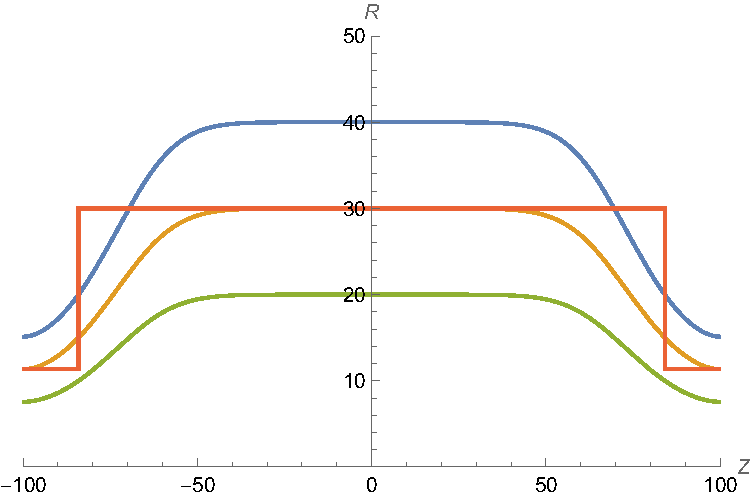
\includegraphics{SquareWell.pdf}
\caption{An example plot of field lines and the square-well approximation to the central field line}
\label{squarewellplot}
\end{figure}

\subsection{The Centrifugal Potential}

Many results have been derived for confinement in mirror machines which possess an electrostatic potential that varies along the field line. We can make use of these results by noting the following fact: the potential energy of a charged particle on a rotating field line at radius $R$ with angular velocity $\omega$ is
\begin{equation}
\Xi_s = Z_s e \pot - \frac{m_s}{2} \omega^2 R^2.
\end{equation}
We can thus reuse results from existing papers simply by making the substitution $Z_s e\pot \rightarrow \Xi_s$.

Physically, this electrostatic potential exists to keep the electrons (which are light and barely affected by the centrifugal force) next to the ions which are pushed to regions of large $R$ by the centrifugal force.
Hence, the potential $\pot$ has to be solved for by insisting that the plasma is quasineutral along field lines (and that the loss rate is ambipolar).
If we assume that the plasma rotates at a large Mach number $M \gg 1$, then the plasma is well-confined and the confinement time is long compared to the collision time (this can be checked \textit{a posteriori}). In such a situation the plasma is locally Maxwellian (equivalently it is in LTE) and we can write the density of species $s$ as~\cite{catto:2784,flowtome1}:
\begin{equation}
n_s = N_s(\psi) \exp\left( - \frac{\Xi_s}{T_s} \right).
\label{confinedDensity}
\end{equation}
If we now insist that the plasma is made up of ions (mass $m_i$ and charge $Z_i e$) and electrons (mass $m_e$ and charge $-e$) then quasineutrality reads
\begin{equation}
Z_i N_i \exp\left( - \frac{Z_i e\pot}{T_i} + \frac{m_i}{2T_i} \omega^2 R^2 \right) = N_e \exp\left( \frac{e\pot}{T_e} + \frac{m_e}{2T_e} \omega^2 R^2 \right).
\end{equation}
Without loss of generality, we can pick a baseline for $\pot$ such that $Z_i N_i = N_e$ (to see this, average along a field line, use the fact that neither $N_s$ nor $T_s$ varies along the field line). Furthermore, by neglecting the term containing the electron mass, we can solve the resulting equation for $\pot$:
\begin{equation}
\pot = \left( \frac{Z_i e}{T_i} + \frac{e}{T_e}\right)^{-1} \frac{m_i}{2 T_i} \omega^2 R^2,
\end{equation}
up to a possible constant offset. It is clear that this potential is $\Or(M^2T_e/e)$ and is, in fact, the leading order term in an asymptotic series in $M^{-1}$.\footnote{In computing the densities in \eref{confinedDensity}, we have integrated over a full Maxwellian distribution, neglecting the fact that some small number of high-energy particles are in fact lost alongt he field line. This is a consistent approximation as we have determined that the potential barrier is $\Or(M^2T_e)$, which to leading order is effectively infinite.} 
To compute the next-order terms in this series we need to know about lost particles and hence parallel transport. This is tackled in the next section. We end with a convenient expression for the potential drop from the centre of a flux surface (at $R = R_{max}$) in terms of suitably normalized variables:

\begin{equation}
\frac{e \pot}{T_e} = \left( \frac{Z_i}{\tau} + 1 \right)^{-1} \frac{M^2}{2} \left( \frac{R^2}{R_{\mathrm{max}}^2 - 1 \right),
\end{equation}
where we $\tau = T_i/T_e$ and we have defined the sonic Mach number $M = \omega R_{max} / \cs$ in terms of the sound speed $\cs^2 = T_e / m_i$.\footnote{This is not the speed at which sound waves propagate in a warm plasma, but provides a very convenient normalization. It is the cold-ion limit of the sound speed, and we will continue to call it the sound speed despite this abuse of terminology.}
If $Z_i = \tau = 1$ then we get the usual $M^2/4$ scaling for the potential drop. It is also useful to note that, as a consequence of flux conservation
	\begin{equation}
	\frac{B_{\mathrm{min}}}{B_{\mathrm{max}}} = \left(\frac{R_{\mathrm{max}}}{R_{\mathrm{min}}}\right)^2
	\label{<+label+>}
\end{equation}<++>

\subsection{Parallel Transport}

We assume that the plasma is hot enough to be in the collisionless regime where the particle bounce time (inside the potential well formed by the centrifugal force) is extremely short compared to the particle collision time. This is manifestly true in reactor-grade plasmas ($\left.\nu_{ii} L_\parallel \right/ \vth \sim 10^{-5}$ or smaller) but is even valid for warm plasmas above a few hundred electron Volts in temperature. The collisionality parameter is reported and if it is not much less than one the results of \mctrans{} are not valid.

In this collisionless regime we use formulae that are derived in the manner originally used by Pastukhov~\cite{Pastukhov1974} for the case of a tandem mirror with an electron-confining electrostatic potential. Pastukhov originally derived his results for electrons alone. We need the result for a multispecies plasma.  
We can find this result in \citet{CattoBernsteinMirror1} by taking the square-well limit of .

\subsection{Perpendicular Transport}

\subsection{Alpha Particles and Nuclear Physics}
Our fundamental model for alpha particles is that they are all born with a delta-function distribution at the birth energy of $E_\alpha = 3.52$ MeV:
\begin{equation}
\left( \pd{f_\alpha}{t}\right)_{\mathrm{Source}} = \frac{S_\alpha \delta(v-v_*)}{4\pi v_*^2}
\end{equation}
where $v_*$ is the birth velocity corresponding to $E_\alpha$ and $S_\alpha$ is the birth rate of alphas per unit time per unit volume.
\subsubsection{Prompt Alpha Losses}
Alpha particles are born isotropically. Thus, a fraction of them are born directly into the unconfined region of velcoity space.
The birth energy of alphas $E_\alpha$ is much greater than the centrifugal potential which is roughly $M^2 T_e / 4$ (at fusion temperatures and parameters this remains
less than $0.5$ MeV). We thus model the 
\subsubsection{Collisional Alpha Losses}
\subsubsection{Alpha Heating}

\subsection{Neutral Transport}
We currently have no model of transport due to neutral particles. A first step towards this will be implementing a diagnostic for 
the neutral mean free path in our plasma. In the limit of either very small or very long mean free path, we may be able to make further approximations to evaluate the 
losses from charge exchange.

\textbf{N.B. Until more neutral physics is implemented, we have no way to handle self-consistent fuelling scenarios. The only reasonable assumption
	is that losses due to neutrals are small and feedback control is used to target a fixed electron density.}

\subsection{Radiative Processes and Impurities}
There are two ways to model impurities in \mctrans{}. Firstly is a ``lumped impurity'' that only changes the effective charge state $Z_{\mathrm{eff}}$ and 
provides \textit{only} bremsstrahlung radiation. It does not dilute the main ion species, so quasineutrality is enforced by only considering the main ions and 

\subsubsection{Bremsstrahlung and Synchrotron Radiation}
\subsubsection{Line Radiation}
 Without a better model for the impurity 
species that are present (including multiple charge states) we cannot reliably predict the amount of line radiation lost from the plasma.

\textbf{N.B. Because of the lack of ionization and radiative cooling, one should view low-temperature outputs from \mctrans{} extremely sceptically!}


\appendix
\section{Full Syntax for \mctrans{} configuration files}
\section{References}
\bibliographystyle{apsrev}
\bibliography{references}
\end{document}

